\chapter{Algebraic expressions}
\fancyfoot[LO,RE]{Focus Area: Mathematics}

% \setcounter{figure}{1}
% \setcounter{subfigure}{1}
% 
% A number is a way of representing quantity. The numbers used in high school are all real numbers, but there are many different ways of writing any single real number.\par 
% This section describes rational and irrational numbers.\par 

% \setcounter{subfigure}{0}
% \begin{figure}[H] % horizontal\label{m38348*circuits-1}
% Khan Academy video on Integers and Rational Numbers\vspace{.1in} \nopagebreak
% \label{m38348*yt-media1}\label{m38348*yt-video1}
% \raisebox{-5 pt}{ 
\includegraphics[width=0.5cm]{col11306.imgs/summary_www.png}} { (Video:  MG10034 )}
% \vspace{2pt}
% \vspace{.1in}
% \end{figure}       

% \par 
% \subsection*{The big picture of numbers}
% \addcontentsline{toc}{subsection}{The big picture of numbers}


\setcounter{subfigure}{0}
\begin{figure}[H] % horizontal\label{m38348*id62548}
\begin{center}
% \label{m38348*id62548!!!underscore!!!media}\label{m38348*id62548!!!underscore!!!printimage}
%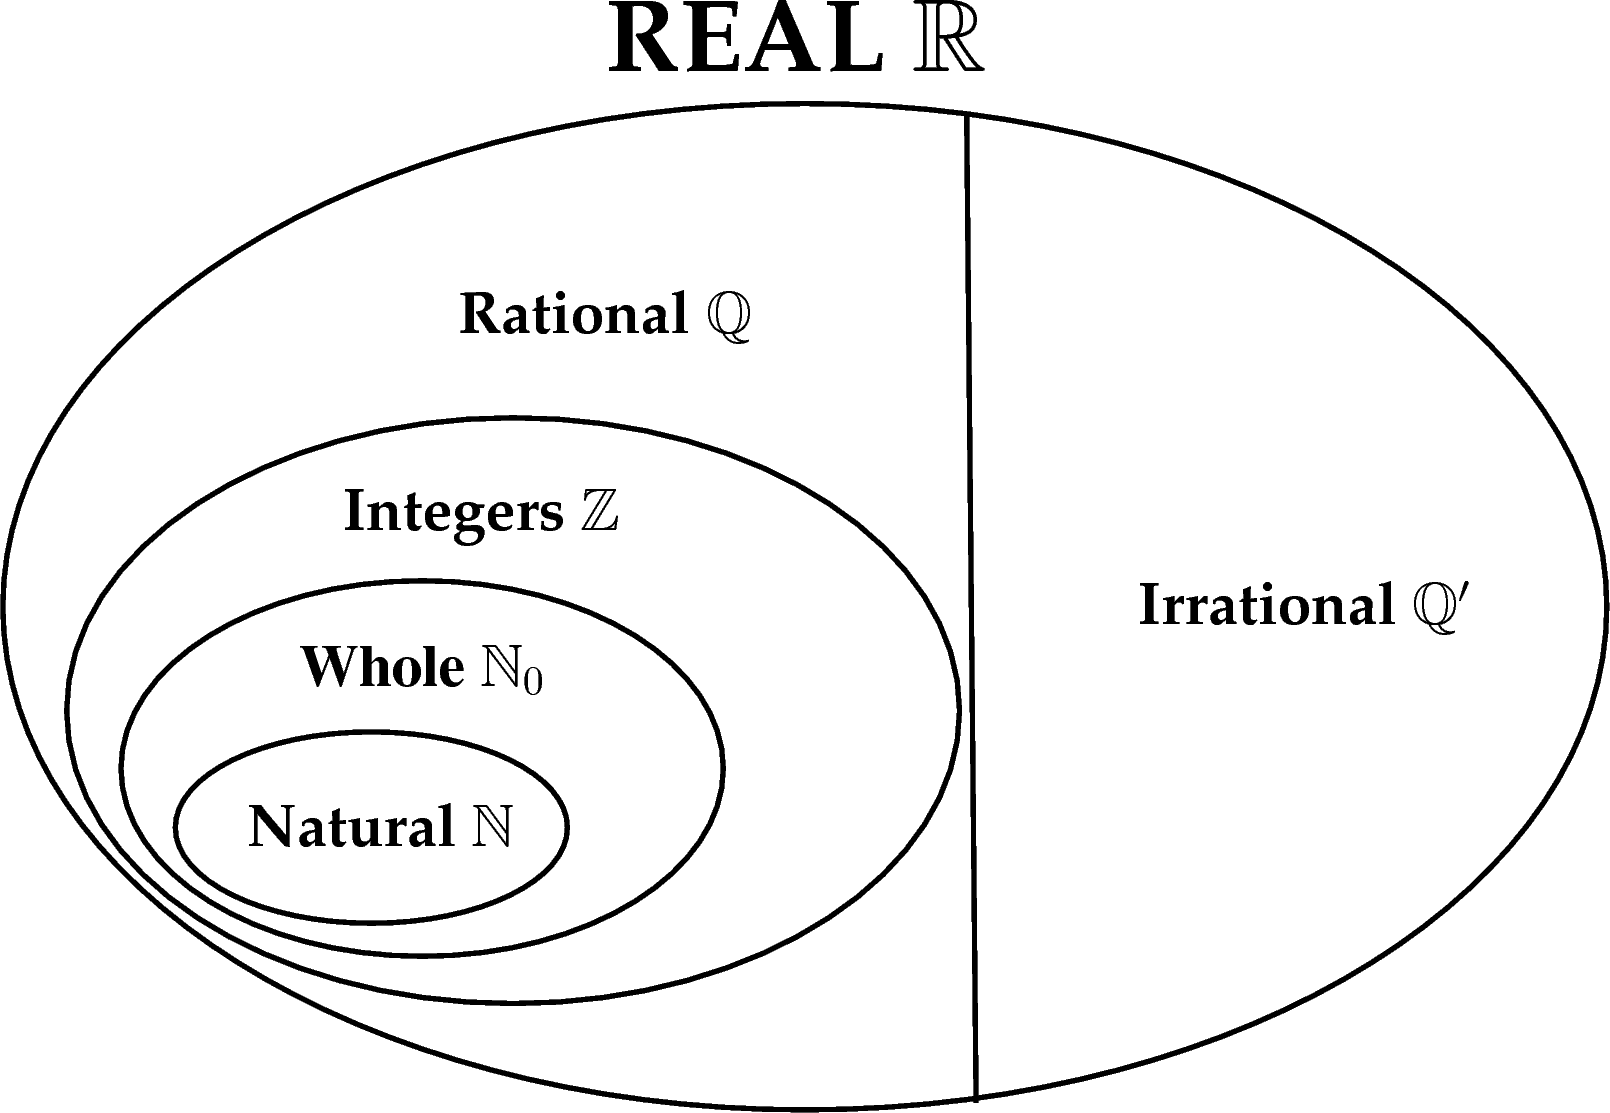
\includegraphics[width=9cm]{col11306.imgs/m38348_MG10C3_001.png} % m38348;MG10C3\_001.png;;;6.0;8.5;
\scalebox{0.6} % Change this value to rescale the drawing.
{
\begin{pspicture}(0,-4.764375)(14.481563,4.804375)
\psellipse[linewidth=0.04,dimen=outer](6.81,-0.484375)(6.81,4.28)
\psline[linewidth=0.04cm](8.18,3.695625)(8.26,-4.684375)
\psellipse[linewidth=0.04,dimen=outer](4.34,-1.364375)(3.8,2.5)
\psellipse[linewidth=0.04,dimen=outer](3.57,-1.854375)(2.57,1.61)
% \usefont{T1}{ppl}{b}{n}
\rput(6.735781,4.350625){\Huge Real $\mathbb{R}$}
% \usefont{T1}{ppl}{b}{n}
\rput(11.03875,-0.484375){\Huge Irrational $\mathbb{Q'}$}
% \usefont{T1}{ppl}{b}{n}
\rput(5.11875,1.975625){\Huge Rational $\mathbb{Q}$}
% \usefont{T1}{ppl}{b}{n}
\rput(4.06875,0.275625){\Huge Integer $\mathbb{Z}$}
% \usefont{T1}{ppl}{b}{n}
\rput(3.21875,-2.324375){\Huge Natural $\mathbb{N}$}
\psellipse[linewidth=0.04,dimen=outer](3.14,-2.354375)(1.68,0.83)
% \usefont{T1}{ptm}{b}{n}
\rput(3.5735939,-1.024375){\Huge Whole $\mathbb{N}_0$}
\end{pspicture} 
}
\vspace{2pt}
\vspace{.1in}
\end{center}
\end{figure}       
\par 
We use the following definitions:\par 
\begin{itemize}[itemsep=5pt]
\item $\mathbb{N}$: natural numbers are $\{1;~2;~3;~\ldots\}$
\item $\mathbb{N}_0$: whole numbers are $\{0;~1;~2;~3;~\ldots\}$
\item $\mathbb{Z}$: integers are $\{\ldots;~-3;~-2;~-1;~0;~1;~2;~3;~\ldots\}$
\end{itemize}
\par
\chapterstartvideo{VMabo}

\section{Rational and irrational numbers}

\Definition{Rational number}
{A rational number ($\mathbb{Q}$) is any number which can be written as: 
%       \label{m38348*uid6}\nopagebreak\noindent{}

\begin{equation*}
\frac{a}{b}
\end{equation*}
where $a$ and $b$ are integers and $b\ne 0$. \par 
} 
\par

The following numbers are all rational numbers:\par 


\begin{equation*}
\frac{10}{1};~\frac{21}{7};~\frac{-1}{-3};~\frac{10}{20};~\frac{-3}{6}
\end{equation*}
We see that all numerators and all denominators are integers.

This means that all integers are rational numbers, because they can be
written with a denominator of $1$.\\


% \subsection{Irrational numbers}
% \setcounter{figure}{1}
% \setcounter{subfigure}{1}


% Writing numbers to many decimal places or a high accuracy is very inconvenient and rarely gives practical answers. For this reason we often estimate the number to a certain number of decimal places.\par 

\Definition{Irrational numbers}{Irrational numbers ($\mathbb{Q'}$) are numbers that cannot be written as a fraction with the numerator and denominator as integers.

%  This means that any number that is not a terminating or recurring decimal number is irrational. 
}

Examples of irrational numbers:\par 

\begin{equation*}
  \sqrt{2};~\sqrt{3};~\sqrt[3]{4};~\pi;~\frac{1+\sqrt{5}}{2}
\end{equation*}

These are not rational numbers, because either the numerator or the denominator is not an integer.\par 

% \Tip{When irrational numbers are written in decimal form, they go on forever and
% there is no repeated pattern of digits. \\The square roots of non-perfect squares and the cube roots of non-perfect cubes are all irrational.}


% \begin{activity}{Irrational numbers }
% \nopagebreak
% Which of the following cannot be
% written as a rational number?\par \vspace{0.5cm}
% \textbf{Remember}: A rational number is a fraction with numerator and denominator as integers. Terminating decimal numbers or recurring decimal numbers are rational.\par 
% \begin{enumerate}[itemsep=5pt, label=\textbf{\arabic*}. ] 
% \item $\pi =3,14159265358979323846264338327950288419716939937510\ldots$
% \item $1,4$
% \item $1,618033989\ldots$
% \item $100$
% \item $1,7373737373\ldots$
% \item $0,\overline{02}$
% \end{enumerate}
% \end{activity}

% Consider
% \begin{equation*}
% \frac{\sqrt{2}}{7};~\frac{20}{\pi}
% \end{equation*}
% These are not rational numbers, because either the numerator or the denominator is not an integer.\par 
% A number may not be written as an integer divided by another integer, but may still
% be a rational number. The rule is, if a number can be written
% as a fraction of integers, it is rational even if it can be written in other
% ways as well. These two examples might not look like rational numbers
% at first glance, but because there have equivalent forms that can be expressed as an
% integer divided by another integer, they are rational:\par 
% \nopagebreak\noindent{}
% \begin{equation*}    
% \frac{-1,33}{-3}=\frac{133}{300}; ~~~~~~\frac{-3}{6,39}=\frac{-300}{639}=\frac{-100}{213}
% \end{equation*}

\subsection*{Decimal numbers}
\addcontentsline{toc}{subsection}{Decimal numbers}
\nopagebreak
All integers and fractions with integer numerators and denominators are rational numbers. %There are two more forms of rational numbers.
\par 
 
% \begin{activity}{Decimal numbers }
% \nopagebreak
% You can write the rational number
% $\frac{1}{2}$ as the decimal number $0,5$. Write the following numbers as
% decimals:\par 
% \begin{enumerate}[itemsep=5pt, label=\textbf{\arabic*}. ] 
% \item $\dfrac{1}{4}$
% \item $\dfrac{1}{10}$
% \item $\dfrac{2}{5}$
% \item $\dfrac{1}{100}$
% \item $\dfrac{2}{3}$
% \end{enumerate}
% Do the digits after the decimal comma end or do they continue? If they continue, is there a recurring pattern to the digits? \par 
% \end{activity}

You can write any rational number as a decimal number but not all
decimal numbers are rational numbers. These types of decimal
numbers are rational numbers:\par 
\begin{itemize}
\item Decimal numbers that end (or terminate). For example, the fraction $\dfrac{4}{10}$ can be written as $0,4$.
\item Decimal numbers that have a repeating single digit. For example, the fraction $\dfrac{1}{3}$ can be written as 
$0,\dot{3}$ or as $0,\bar{3}$. 
The dot and bar notations are equivalent and both represent recurring $3$'s, i.e.
$0,\dot{3} = 0,\bar{3} = 0,333\ldots$.
\item Decimal numbers that have a recurring pattern of multiple digits. For example, the fraction $\dfrac{2}{11}$ can also be written as 
$0,\overline{18}$. 
The bar represents a recurring pattern of $1$ and $8$'s i.e.
$0,\overline{18} = 0,181818\ldots$.
\end{itemize}

\par
\textbf{Notation:} You can use a dot or a bar over the repeated numbers to indicate that the decimal is a recurring decimal. If the bar covers more than one number, then all numbers beneath the bar are recurring.

\par
If you are asked to identify whether a number is rational or
irrational, first write the number in decimal form. If the number
terminates then it is rational. If it goes on forever, then look for a
repeated pattern of digits. If there is no repeated pattern, then the
number is irrational.
 
\par
When you write irrational numbers in decimal form, you may continue writing them for many, many
decimal places. However, this is not convenient and it is often necessary to round off.


\begin{wex}{Rational and irrational numbers}
{Which of the following are not rational numbers?\\
\begin{enumerate}[itemsep=5pt, label=\textbf{\arabic*}. ] 
\item $\pi =3,14159265358979323846264338327950288419716939937510\ldots$
\item $1,4$
\item $1,618033989\ldots$
\item $100$
\item $1,7373737373\ldots$
\item $0,\overline{02}$
\end{enumerate}}
{
\begin{enumerate}[itemsep=5pt, label=\textbf{\arabic*}. ] 
\item Irrational, decimal does not terminate and has no repeated pattern. 
\item Rational, decimal terminates.
\item Irrational, decimal does not terminate and has no repeated pattern. 
\item Rational, all integers are rational.
\item Rational, decimal has repeated pattern.
\item Rational, decimal has repeated pattern.
\end{enumerate}
}
\end{wex}

\subsection{Converting terminating decimals into rational numbers}

% \addcontentsline{toc}{subsection}{Converting terminating decimals into rational numbers}
A decimal number has an integer part and a fractional part. For example, $10,589$ has an integer part of $10$ and a fractional part of $0,589$ because $10+0,589=10,589$. The fractional part can be written as a rational number, i.e.\@{} with a numerator and denominator that are integers. \\
\\
Each digit after the decimal point is a fraction with a denominator in increasing powers of $10$.\\ For example,
\begin{itemize}
\item $0,1$ is $\dfrac{1}{10}$
\item $0,01$ is $\dfrac{1}{100}$
\item $0,001$ is $\dfrac{1}{1~000}$
\end{itemize}

This means that
\begin{align*}
  10,589 &= 10 + \dfrac{5}{10} + \dfrac{8}{100} + \dfrac{9}{1~000} \\
  &= \dfrac{10~000}{1~000} + \dfrac{500}{1~000} + \dfrac{80}{1~000} + \dfrac{9}{1~000} \\
  &= \dfrac{10~589}{1~000} \\
\end{align*}

\subsection{Converting recurring decimals into rational numbers}


When the decimal is a recurring decimal, a bit more work is needed to write the fractional part of the decimal number as a fraction.\par 

\begin{wex}
{%title
Converting decimal numbers to fractions
}
{%question
Write $0,\dot{3}$ in the form $\dfrac{a}{b}$ (where $a$ and $b$ are integers).
}
{%answer

\westep{Define an equation}
$$\mbox{Let } x = 0,33333\ldots$$

\westep{Multiply by $10$ on both sides}
$$10x = 3,33333\ldots$$

\westep{Subtract the first equation from the second equation}
$$9x = 3 $$

\westep{Simplify}
$$ x = \dfrac{3}{9} = \dfrac{1}{3} $$
}
\end{wex}


\begin{wex}
{%title
Converting decimal numbers to fractions
}
{%question
Write $5,\dot{4}\dot{3}\dot{2}$ as a rational fraction.
}
{%answer

\westep{Define an equation}
$$ x = 5,432432432\ldots $$

\westep{Multiply by $1000$ on both sides}
$$ 1~000x = 5~432,432432432\ldots $$

\westep{Subtract the first equation from the second equation}
$$ 999x = 5~427 $$

\westep{Simplify}
$$ x = \dfrac{5~427}{999} = \dfrac{201}{37} = 5\dfrac{16}{37}$$
}
\end{wex}

In the first example, the decimal was multiplied by $10$ and in the
second example, the decimal was multiplied by $1~000$. This is because
there was only one digit recurring (i.e. $3$) in the first example,
while there were three digits recurring (i.e. $432$) in the second
example.\par 

In general, if you have one digit recurring, then multiply by $10$. If
you have two digits recurring, then multiply by $100$. If you have
three digits recurring, then multiply by $1~000$ and so on.\par

Not all decimal numbers can be written as rational numbers. Why? Irrational decimal numbers like 
$\sqrt{2}=1,4142135\ldots$
cannot be written with an integer numerator and denominator, because they do not have a pattern of recurring digits and they do not terminate. However, when possible, you should try to use rational numbers or fractions instead of decimals.
% \label{m38348*secfhsst!!!underscore!!!id606}




\begin{exercises}{}{
\begin{enumerate}[itemsep=5pt, label=\textbf{\arabic*}. ] 
\item State whether the following numbers are $\mathbb{Q}$ or $\mathbb{Q'}$. If the number is $\mathbb{Q}$, state whether it is $\mathbb{N}_0$, $\mathbb{N}$ or $\mathbb{Z}$:
\begin{enumerate}[itemsep=5pt, label=\textbf{(\alph*)} ] 
    \item $-\dfrac{1}{3}$
    \item $0,651268962154862\ldots$
    \item $\dfrac{\sqrt{9}}{3}$
    \item $\pi^2$
\end{enumerate}
\item If $a$ is an integer, $b$ is an integer and $c$ is irrational, which of the following are rational numbers? 
  \begin{enumerate}[itemsep=5pt, label=\textbf{(\alph*)} ] 
    \item $\dfrac{5}{6}$
    \item $\dfrac{a}{3}$
    \item $\dfrac{-2}{b}$
    \item $\dfrac{1}{c}$
    \end{enumerate}
\item For which of the following values of $a$ is $\frac{a}{14}$ rational or irrational?
    \begin{enumerate}[itemsep=0pt, label=\textbf{(\alph*)} ] 
    \item $1$
    \item $-10$
    \item $\sqrt{2}$
    \item $2,1$
    \end{enumerate}
%         \end{enumerate}
% \par 
%  \par \begin{tabular}[h]{cccccc}
%  (1.) l35  &  (2.) l3N  & \end{tabular}}
% \end{exercises}
% 
%            \begin{exercises}{Fractions }{
%             \nopagebreak
%       \label{m38348*id63882}\begin{enumerate}[itemsep=5pt, label=\textbf{\arabic*}. ] 
\item Write the following as fractions:
    \begin{enumerate}[itemsep=0pt, label=\textbf{(\alph*)} ] 
    \item $0,1$
    \item $0,12$
    \item $0,58$
    \item $0,2589$
    \end{enumerate}
%         \end{enumerate}
% \par 
%  \par \begin{tabular}[h]{cccccc}
%  (1.) l3R  & \end{tabular}}
% \end{exercises}
% 
% \begin{exercises}{Repeated Decimal Notation }{
% %             \nopagebreak
%       \label{m38348*id64513}\begin{enumerate}[itemsep=5pt, label=\textbf{\arabic*}. ] 
\item Write the following using the recurring decimal notation:
    \begin{enumerate}[itemsep=0pt, label=\textbf{(\alph*)} ] 
    \item $0,11111111\ldots$
    \item $0,1212121212\ldots$
    \item $0,123123123123\ldots$
    \item $0,11414541454145\ldots$
    \end{enumerate}
\item Write the following in decimal form, using the recurring decimal notation:
    \begin{enumerate}[itemsep=5pt, label=\textbf{(\alph*)} ] 
    \item $\dfrac{2}{3}$
    \item $1\dfrac{3}{11}$
    \item $4\dfrac{5}{6}$
    \item $2\dfrac{1}{9}$
    \end{enumerate}
\item Write the following decimals in fractional form:
    \begin{enumerate}[itemsep=3pt, label=\textbf{(\alph*)} ] 
    \item $0,\dot{5}$
    \item $0,6\dot{3}$
    \item $5,\overline{31}$
    \end{enumerate}
\end{enumerate}
\practiceinfo 
\par 
 \par \begin{tabular}[h]{cccccc}
 (1.) 023j & (2.) 00bb&  (3.) 00bc&  (4.) 00bd& (5.) 00be& (6.) 00bf& (7.) 00bg\end{tabular}
}
\end{exercises}

\section{Rounding off}
\nopagebreak
%%$ \hspace{-5pt}\begin{array}{cccccccccccc}   
\includegraphics[width=0.75cm]{col11306.imgs/summary_fullmarks.png} &   \end{array} $ \hspace{2 pt}\raisebox{-5 pt}{} {(section shortcode: MG10057 )} \par 
Rounding off a decimal number to a given number of decimal places is
the quickest way to approximate a number. For example, if you wanted
to round off $2,6525272$ to three decimal places, you would:
\begin{itemize}
\item count three places after the decimal and place a $|$ between the third and fourth numbers
\item round up the third digit if the fourth digit is greater than or equal to $5$
\item leave the third digit unchanged if the fourth digit is less than $5$
\item if the third digit is $9$ and needs to be round up, then the $9$ becomes a $0$ and the second digit rounded up
\end{itemize}
\par 
So, since the first digit after the $|$ is a $5$, we must round up the digit in the third decimal place to a $3$ and the final answer of $2,6525272$ rounded to three decimal places is $2,653$.
\par


\begin{wex}{Rounding off }

{Round off the following numbers to the indicated number of decimal places: 
\begin{enumerate}[itemsep=5pt, label=\textbf{\arabic*}. ] 

\item $\frac{120}{99}=1,\dot{1}\dot{2}$ to $3$ decimal places.
\item $\pi =3,141592653\ldots$ to $4$ decimal places.
\item $\sqrt{3}=1,7320508\ldots$ to $4$ decimal places.
\item $2,78974526$ to $3$ decimal places.
\end{enumerate}
}
{
\westep{Mark off the required number of decimal places}

\begin{enumerate}[itemsep=5pt, label=\textbf{\arabic*}. ] 
\item $\frac{120}{99}=1,212|121212\ldots$
\item $\pi =3,1415|92653\ldots$
\item $\sqrt{3}=1,7320|508\ldots$
\item $2,789|74526$
\end{enumerate}

\westep{Check the next digit to see if you must round up or round down}
\begin{enumerate}[itemsep=5pt, label=\textbf{\arabic*}. ]
\item The last digit of $\frac{120}{99}=1,212|121212\dot{1}\dot{2}$  must be rounded down.
\item The last digit of $\pi =3,1415|92653\ldots$ must be rounded up.
\item The last digit of $\sqrt{3}=1,7320|508\ldots$ must be rounded up.
\item  The last digit of $2,789|74526$ must be rounded up.
\newline Since this is a $9$, we replace it with a $0$ and round up the second last digit.
\end{enumerate}

\westep{Write the final answer}
\begin{enumerate}[itemsep=5pt, label=\textbf{\arabic*}. ]
\item $\frac{120}{99}=1,212$ rounded to $3$ decimal places.
\item $\pi =3,1416$  rounded to $4$ decimal places.
\item $\sqrt{3}=1,7321$ rounded to $4$ decimal places.
\item $2,790$.
\end{enumerate}
}  
\end{wex}



\begin{exercises}{}
{Use your calculator to write the following in decimal form, rounded to $3$ decimal places:
\begin{enumerate}[itemsep=3pt, label=\textbf{\arabic*}. ]
\item $12,56637061\ldots$ %$4\pi$
\item $3,31662479\ldots$ %$\sqrt{11}$
\item $0,26666666\ldots$ %$\dfrac{0,8}{3}$
\item $1,912931183\ldots$ %$\sqrt[3]{7}$
\item $6,32455532\ldots$ %$2\sqrt{10}$
\item $0,05555555\ldots$ %$\dfrac{1}{18}$
\end{enumerate}
\practiceinfo 
\par 
 \par \begin{tabular}[h]{c}
 (1.-6.) 00bh\end{tabular}
}

\end{exercises}


\section{Estimating surds}
\setcounter{figure}{1}
\setcounter{subfigure}{1}
If the ${n}^{\mathrm{th}}$ root of a number cannot be simplified to a rational number, we call it a surd. For example, $\sqrt{2}$ and $\sqrt[3]{6}$ are surds, but $\sqrt{4}$ is not a surd because it can be simplified to the rational number $2$.\par 
In this chapter we will look at surds of the form $\sqrt[n]{a}$ where $a$ is any positive number, for example, $\sqrt{7}$ or $\sqrt[3]{5}$. It is very common for $n$ to be $2$, so we usually do not write $\sqrt[2]{a}$. Instead we write the surd as just $\sqrt{a}$.\par 
It is sometimes useful to know the approximate value of a surd without having to use a calculator. For example, we want to be able to estimate where a surd like $\sqrt{3}$ is on the number line. From a calculator we know that $\sqrt{3}$ is equal to $1,73205\ldots$. It is easy to see that $\sqrt{3}$ is above $1$ and below $2$. But to see this for other surds like $\sqrt{18}$ without using a calculator, you must first understand the following:\par 


\Identity{
\begin{center}
If $a$ and $b$ are positive whole numbers, and $a\lessthan{}b$, then $\sqrt[n]{a}\lessthan{}\sqrt[n]{b}$. 
\end{center}}

\par
A perfect square is the number obtained when an integer is squared. For example, $9$ is a perfect square since ${3}^{2}=9$. \\Similarly, a perfect cube is a number which is the cube of an integer. For example, $27$ is a perfect cube, because ${3}^{3}=27$.
\par
Consider the surd $\sqrt[3]{52}$. It lies somewhere between $3$ and $4$, because $\sqrt[3]{27}=3$ and $\sqrt[3]{64}=4$ and $52$ is between $27$ and $64$. %Checking on a calculator we see that $\sqrt[3]{52}=3,73\ldots$ which is indeed between $3$ and $4$.

\begin{wex}{Estimating surds}
{%question
Find the two consecutive integers such that $\sqrt{26}$ lies between them.
(Remember that consecutive integers are two integers that follow one
another on the number line, for example, $5$ and $6$ or $8$ and $9$).
}
{%answer

\westep{Use perfect squares to estimate the lower integer}     
${5}^{2}=25$. Therefore $5\lessthan{}\sqrt{26}$.

\westep{Use perfect squares to estimate the upper integer}
${6}^{2}=36$. 
Therefore $\sqrt{26}\lessthan{}6$.

\westep{Write the final answer}
$5\lessthan{}\sqrt{26}\lessthan{}6$. 
}
\end{wex}


\begin{wex}{Estimating surds}
{%
Find the two consecutive integers such that $\sqrt[3]{49}$ lies between them.
}
{%

\westep{Use perfect cubes to estimate the lower integer}   ${3}^{3}=27$, therefore $3\lessthan{}\sqrt[3]{49}$.

\westep{Use perfect cubes to estimate the upper integer} ${4}^{3}=64$, therefore $\sqrt[3]{49}\lessthan{}4$. 

\westep{Write the answer}
$3\lessthan{}\sqrt[3]{49}\lessthan{}4$

\westep{Check the answer by cubing all terms in the inequality and then simplify}
$27<49<64$. This is true, so $\sqrt[3]{49}$ lies between $3$ and $4$.
}
\end{wex}

\begin{exercises}{}
{Determine between which two consecutive integers the following numbers lie, without using a calculator:
\begin{enumerate}[itemsep=0pt, label=\textbf{\arabic*}. ]
\item $\sqrt{18}$
\item $\sqrt{29}$
\item $\sqrt[3]{5}$
\item $\sqrt[3]{79}$

\end{enumerate}
\practiceinfo 
\par 
 \par \begin{tabular}[h]{c}
 (1.-4.) 00bi\end{tabular}
}
\end{exercises}



\section{Products}
\setcounter{figure}{1}
\setcounter{subfigure}{1}
%% $ \hspace{-5pt}\begin{array}{cccccccccccc}   
\includegraphics[width=0.75cm]{col11306.imgs/summary_fullmarks.png} &   \end{array} $ \hspace{2 pt}\raisebox{-5 pt}{} {(section shortcode: MG10060 )} \par 
%   
\nopagebreak
Mathematical expressions are just like sentences and their parts have special names. You should be familiar with the following words used to describe the parts of  mathematical expressions.\par 

\begin{equation*}
3x^2 + 7xy - 5^3 = 0
\end{equation*}



\begin{table}[H]
\begin{center}
\begin{tabular}{|l|l|}
\hline
\textbf{Name} & \textbf{Examples} \\
\hline
term & $3x^2;~7xy;~-5^3$\\ \hline
expression & $3x^2 + 7xy -5^3$\\ \hline
coefficient & $3;~7$\\ \hline
exponent & $2;~1;~3$\\ \hline
base & $x;~y;~5$\\ \hline
constant & $3;~7$\\ \hline
variable & $x;~y$\\ \hline
equation & $3x^2 + 7xy -5^3 = 0$\\ \hline

% \label{m39387*secfhsst!!!underscore!!!id1562}\vspace{.5cm}

\end{tabular}
\end{center}
\end{table} 

\par

\subsection*{Multiplying a monomial and a binomial}

A monomial is an expression with one term, for example, $3x$ or $y^2$.
A binomial is an expression with two terms, for example,
$ax+b$ or $cx+d$.

\begin{wex}{Simplifying brackets}
{Simplify: $2a(a-1) - 3(a^{2}-1)$.}
{
\begin{align*}
  2a(a-1) -3(a^{2}-1) &= 2a(a) + 2a(-1) + (-3)(a^{2})+(-3)(-1) \\
  &= 2a^{2} - 2a - 3a^{2} + 3 \\
  &= -a^{2} -2a + 3
\end{align*}
}
\end{wex}

\subsection*{Multiplying two binomials}

Here we multiply (or expand) two linear binomials:

\begin{center}
\scalebox{1} % Change this value to rescale the drawing.
{
\begin{pspicture}(0,-0.93)(2.8490624,0.93)
\usefont{T1}{ptm}{m}{n}
\rput(1.3745313,-0.03){\LARGE$(ax+b)(cx+d)$}
\psbezier[linewidth=0.02,arrowsize=0.05291667cm 2.0,arrowlength=1.4,arrowinset=0.4]{<-}(1.61,0.16)(1.45,0.66)(0.5260656,0.6082759)(0.47,0.16)
\psbezier[linewidth=0.02,arrowsize=0.05291667cm 2.0,arrowlength=1.4,arrowinset=0.4]{<-}(2.33,0.2)(2.05,0.92)(0.6014754,0.7481931)(0.51,0.2576)
\psbezier[linewidth=0.02,arrowsize=0.05291667cm 2.0,arrowlength=1.4,arrowinset=0.4]{->}(1.17,-0.26705882)(1.25,-0.7)(1.71,-0.5917647)(1.75,-0.24)
\psbezier[linewidth=0.02,arrowsize=0.05291667cm 2.0,arrowlength=1.4,arrowinset=0.4]{->}(0.51,-0.2)(0.69,-0.8428571)(2.07,-0.92)(2.39,-0.27714285)
% \usefont{T1}{ptm}{m}{n}
% \rput(0.94453126,0.33)
% \usefont{T1}{ptm}{m}{n}
% \rput(1.8645313,0.35)
% \usefont{T1}{ptm}{m}{n}
% \rput(1.44,-0.37)
% \usefont{T1}{ptm}{m}{n}
% \rput(2.0445313,-0.37)
\end{pspicture}
}
\end{center}
\clearpage

\begin{align*}
  (ax+b)(cx+d) &= (ax)(cx)+(ax)d+b(cx)+bd \\
               &= ac{x}^{2}+adx +bcx+bd \\
               &= ac{x}^{2}+x(ad+bc)+bd
\end{align*}

%\Note{You may use FOIL = F(firsts) O(outers) I(inners) L(lasts) to remember this technique:


\begin{wex}{Multiplying two binomials }
{Find the product: $(3x-2)(5x+8)$. }
{
\begin{align*}
  (3x-2)(5x+8) &= (3x)(5x)+(3x)(8)+(-2)(5x)+(-2)(8) \\
  &= 15{x}^{2}+24x-10x-16 \\
  &= 15{x}^{2}+14x-16
\end{align*}
} 
\end{wex}




The product of two identical binomials is known as the square of the binomial and is written as:

\begin{equation*}
{(ax+b)}^{2}={a}^{2}{x}^{2}+2abx+{b}^{2}
\end{equation*}
If the two terms are of the form $ax+b$, and $ax-b$ then their product is:

\begin{equation*}
(ax+b)(ax-b) ={a}^{2}{x}^{2}-{b}^{2}
\end{equation*}

This product yields the difference of two squares.\par 


\subsection*{Multiplying a binomial and a trinomial}
\addcontentsline{toc}{subsection}{Multiplying a binomial and a trinomial}

% \setcounter{subfigure}{0}


% \begin{figure}[H] % horizontal\label{m39387*productpolynomials}


% \textnormal{Khan Academy video on products of polynomials.}\vspace{.1in} \nopagebreak
% \label{m39387*yt-media1}\label{m39387*yt-video1}
% \raisebox{-5 pt}{ 
\includegraphics[width=0.5cm]{col11306.imgs/summary_www.png}} { (Video:  MG10062 )}

% \end{figure}   

\addtocounter{footnote}{-0}

A trinomial is an expression with three terms, for example, $ax^{2} + bx + c$.
Now we learn how to multiply a binomial and a trinomial.\par 

To find the product of a binomial and a trinomial, multiply out the brackets:\\

\begin{equation*}
  (A+B)(C+D+E)= A(C+D+E)+B(C+D+E) 
\end{equation*}

\par
\mindsetvid{Products of polynomials}{MG10062}
\begin{wex}
{Multiplying a binomial and a trinomial}
{Find the product: $(x-1)({x}^{2}-2x+1)$.} 
{
\westep{Expand the bracket}
$(x-1)(x^2-2x+1) &= x(x^2-2x+1)-1(x^2-2x+1)\\
\phantom{(x-1)(x^2-2x+1)} &= x^3-2x^2+x-x^2+2x-1$
\westep{Simplify}
$\phantom{(x-1)(x^2-2x+1) } = x^3-3x^2 + 3x-1$
}       
\end{wex}



\begin{exercises}{}
{Expand the following products:

\begin{multicols}{2}
\begin{enumerate}[label=\textbf{\arabic*}., itemsep=5pt]
\item $2y(y+4)$ 
\item $(y+5)(y+2) $
\item $(2-t)(1-2t)$
\item $(x-4)(x+4)$
\item $ (2p+9)(3p+1)$
\item $(3k-2)(k+6)$
\item $(s+6)^2$
\item $-(7-x)(7+x)$
\item $(3x-1)(3x+1)$
\item $(7k+2)(3-2k)$
\item $(1-4x)^2$
\item $(-3-y)(5-y)$
\item $(8-x)(8+x)$
\item $(9+x)^2$
\item $(-2{y}^{2}-4y+11)(5y-12)$ 
\item $(7{y}^{2}-6y-8)(-2y+2)$% make-rowspan-placeholders
\item $(10{y}+3)(-2{y}^{2}-11y+2)$ 
\item $(-12y-3)(12{y}^{2}-11y+3)$% make-rowspan-placeholders
\item $(-10)(2{y}^{2}+8y+3)$ 
\item $(2{y}^{6}+3{y}^{5})(-5y-12)$% make-rowspan-placeholders
\item $(-7y+11)(-12y+3)$% make-rowspan-placeholders
\item $(7y+3)(7{y}^{2}+3y+10)$% make-rowspan-placeholders
\item $9(8{y}^{2}-2y+3)$ 
\item $(-6{y}^{4}+11{y}^{2}+3y)(y+4)(y-4)$ 
\end{enumerate}
\end{multicols}
\practiceinfo 
\par 
 \par \begin{tabular}[h]{cccccc}
 (1.-6.) 00bj&  (7.-12.) 00bk&  (13.-18.) 00bm& (19.-24.) 00bn\end{tabular}
}
\end{exercises}



\section{Factorisation}


Factorisation is the opposite process of expanding brackets. For example, expanding brackets would require $2(x+1)$ to be written as $2x+2$. Factorisation would be to start with $2x+2$ and to end up with $2(x+1)$. 

\begin{center}
\scalebox{1} % Change this value to rescale the drawing.
{
\begin{pspicture}(0,-1.1042187)(3.6090624,1.1042187)
% \usefont{T1}{ppl}{m}{n}
\rput(0.78453124,-0.01921875){$2(x+1)$}
\psbezier[linewidth=0.02,arrowsize=0.093cm 2.4,arrowlength=1.4,arrowinset=0.4]{->}(2.85,0.23078126)(2.59,0.9507812)(1.0414754,0.73897433)(0.97,0.27078125)
\psbezier[linewidth=0.02,arrowsize=0.093cm 2.4,arrowlength=1.4,arrowinset=0.4]{->}(0.95,-0.20921876)(1.13,-0.8720759)(2.55,-0.8492187)(2.87,-0.2063616)
% \usefont{T1}{ppl}{m}{n}
\rput(2.8645313,-0.03921875){$2x+2$}
% \usefont{T1}{ptm}{m}{n}
\rput(1.9039062,0.9007813){factorising}
% \usefont{T1}{ptm}{m}{n}
\rput(1.9079688,-1){expanding}
\end{pspicture} 
}
\end{center}

The two expressions $2(x+1)$ and $2x+2$ are equivalent; they have the same value for all values of $x$.
\par
In previous grades, we factorised by taking out a common factor and using difference of squares.\par 
\par
\mindsetvid{Revision of factorisation}{VMabz}

\subsection*{Common factors}

Factorising based on common factors relies on there being factors common to all the terms. \par

For example, $2x-6{x}^{2}$ can be factorised as follows:\par 

\begin{equation*}
2x-6{x}^{2}=2x(1-3x)
\end{equation*}

% \Tip{Check your answer by multiplying the bracket out and make sure you get back to the original expression. 
% \begin{equation*}
%  2x(1-3x) = 2x - 6x^{2}
% \end{equation*}
% is correct.
% }

% 
% \begin{wex}{Factorising }
% {Factorise completely: ${b}^{2}{y}^{5}-3ab{y}^{3}$.}
% {
% \westep{Take out the highest common factor $by^3$}  
% \begin{equation*}
% {b}^{2}{y}^{5}-3ab{y}^{3}& =& b{y}^{3}(b{y}^{2}-3a)
% \end{equation*}
% }
% \end{wex}

\begin{wex}{Factorising using a switch around in brackets }{Factorise: $5(a-2)-b(2-a)$. }
{
Use a ``switch around'' strategy to find the common factor. \\Notice that $2-a = -(a-2)$ 
\begin{align*}
  5(a-2)-b(2-a) &= 5(a-2)-[-b(a-2)] \\
  &= 5(a-2)+b(a-2) \\
  &= (a-2)(5+b)
\end{align*}
}
\end{wex}
% 
% \begin{exercises}{}
% {Find the highest common factors of the following pairs of terms:\par
% 
% \begin{multicols}{2}
% \begin{enumerate}[label=\textbf{\arabic*}., itemsep=5pt]
% \item $6y;~18x$
% \item $12mn;~8n$
% \item $3st;~4su$ 
% \item $18kl;~9kp$
% \item $abc;~ac$% 
% \item $2xy;~4xyz$
% \item $3uv;~6u$ 
% \item $9xy;~15xz$
% \item $24xyz;~16yz$
% \item $3m;~45n$
% \end{enumerate}
% \end{multicols}
% \practiceinfo 
% \par 
%  \par \begin{tabular}[h]{cccccc}
%  (1.-5.) 00bp&  (6.-10.) 00bq\end{tabular}
% }
% \end{exercises}

\subsection* {Difference of two squares}
We have seen that 
\begin{equation*}
(ax+b)(ax-b)~\mbox{ can be expanded to }~{a}^{2}{x}^{2}-{b}^{2}
\end{equation*}

Therefore
\begin{equation*}
{a}^{2}{x}^{2}-{b}^{2}~\mbox{ can be factorised as }~(ax+b)(ax-b)
\end{equation*}
For example, ${x}^{2}-16$ can be written as ${x}^{2}-{4}^{2}$ which is a difference of two squares. Therefore, the factors of ${x}^{2}-16$ are $(x-4)$ and $(x+4)$.

\par
To spot a difference of two squares, look for expressions:
\begin{itemize}
\item consisting of two terms;
\item with terms that have different signs (one positive, one negative);
\item with each term a perfect square.
\end{itemize}
For example, $a^{2}-1$; $4x^{2}-y^{2}$; $-49+p^{4}$.




\begin{wex}{The difference of two squares}
{Factorise: $3a(a^2-4)-7(a^2-4)$.}
{
\westep{Take out the common factor $(a^2-4)$}


\begin{equation*}
  3a(a^2-4)-7(a^2-4) = (a^2-4)(3a-7)
\end{equation*}

\westep{Factorise the difference of two squares $(a^2-4)$ }
$$
(a^2-4)(3a-7) = (a-2)(a+2)(3a-7)
$$
}
\end{wex}


\begin{exercises}{}{Factorise:
\begin{multicols}{2}
\begin{enumerate}[itemsep=5pt, label=\textbf{\arabic*}. ] 
\item $2l+2w$
\item $12x+32y$
\item $6{x}^{2}+2x+10{x}^{3}$
\item $2x{y}^{2}+x{y}^{2}z+3xy$
\item $-2a{b}^{2}-4{a}^{2}b$
\item $7a+4$ 
\item $20a-10$ 
\item $18ab-3bc$
\item $12kj+18kq$ 
\item $16{k}^{2}-4$ 
\item $3{a}^{2}+6a-18$
\item $-12a+24a^3$ 
\item $-2ab-8a$ 
\item $24kj-16{k}^{2}j$
\item $-{a}^{2}b-{b}^{2}a$ 
\item $12{k}^{2}j+24{k}^{2}{j}^{2}$ 
\item $72{b}^{2}q-18{b}^{3}{q}^{2}$
\item $4(y-3)+k(3-y)$ 
\item $a^2(a-1)-25(a-1)$ 
\item $bm(b+4)-6m(b+4)$
\item ${a}^{2}(a+7)+9(a+7)$ 
\item $3b(b-4)-7(4-b)$ 
\item ${a}^{2}{b}^{2}{c}^{2}-1$
\end{enumerate}
\end{multicols}
\practiceinfo 
\par 
 \par \begin{tabular}[h]{cccccc}
 (1.7.) 00br&  (7.-12.) 00bs& (13.-18.) 00bt&  (19.-23.) 00bu\end{tabular}
}
\end{exercises}

\subsection{Factorising by grouping in pairs}

The taking out of common factors is the starting point in all
factorisation problems. We know that the factors of $3x+3$ are $3$
and $(x+1)$. Similarly, the factors of $2{x}^{2}+2x$ are $2x$ and
$(x+1)$. Therefore, if we have an expression
\begin{equation*}
2{x}^{2}+2x+3x+3
\end{equation*}
there is no common factor to all four terms, but we can factorise as
follows:
\begin{equation*}
  (2{x}^{2}+2x)+(3x+3) = 2x(x+1)+3(x+1)
\end{equation*}

We can see that there is another common factor $(x+1)$. Therefore, we can now write:
\begin{equation*}
  (x+1)(2x+3)
\end{equation*}
We get this by taking out the $(x+1)$ and seeing what is left over. We
have $2x$ from the first group and $+3$ from the second group. This is
called factorising by grouping.

%\Tip{Look at the ratios of the coefficients as a guideline for grouping.}


\begin{wex}{Factorising by grouping in pairs}
{Find the factors of $7x+14y+bx+2by$.}
{
\westep{There are no factors common to all terms}

\westep{Group terms with common factors together}

$7$ is a common factor of the first two terms and $b$ is a common
factor of the second two terms. We see that the ratio of the
coefficients $7:14$ is the same as $b:2b$.
\begin{align*}
7x+14y+bx+2by &= (7x+14y)+(bx+2by) \\ 
              &= 7(x+2y)+b(x+2y)
\end{align*}

\westep{Take out the common factor $(x+2y)$}
\begin{equation*}
  7(x+2y)+b(x+2y)=(x+2y)(7+b)
\end{equation*}

% \westep{Write the final answer}  
% The factors of $7x+14y+bx+2by$ are $(7+b)$ and $(x+2y)$.\\
\par
\large{OR}

\westep{Group terms with common factors together}$x$ is a common factor of the first and third terms and $2y$ is a common factor of the second and fourth terms $(7:b~=~14:2b)$.\par 
\westep{Rearrange the equation with grouped terms together}

\begin{align*}
  7x+14y+bx+2by &= (7x+bx)+(14y+2by) \\
  &= x(7+b)+2y(7+b)
\end{align*}

\westep{Take out the common factor $(7+b)$}

\begin{equation*}
x(7+b)+2y(7+b) = (7+b)(x+2y)
\end{equation*}
\westep{Write the final answer}  
The factors of $7x+14y+bx+2by$ are $(7+b)$ and $(x+2y)$.

}
\end{wex}

% There is sometimes more than one correct way to group terms together, as shown in this ercample.

% \begin{wex}
% {Factorising by grouping}
% {Find the factors of $7x+14y+bx+2by$}
% {
% \westep{There are no factors common to all terms}
% 
% \westep{Group terms with common factors together}$x$ is a common factor of the first and third terms and $2y$ is a common factor of the second and fourth terms $(7:b~=~14:2b)$.\par 
% \westep{Rearrange the equation with grouped terms together}
% 
% \begin{align*}
%   7x+14y+bx+2by &= (7x+bx)+(14y+2by) \\
%   &= x(7+b)+2y(7+b)
% \end{align*}
% 
% \westep{Take out the common factor $(7+b)$}
% 
% \begin{equation*}
% x(7+b)+2y(7+b) = (7+b)(x+2y)
% \end{equation*}
% \westep{Write the final answer}  
% The factors of $7x+14y+bx+2by$ are $(7+b)$ and $(x+2y)$.
% }
% \end{wex}

% \setcounter{subfigure}{0}
% \begin{figure}[H] % horizontal\label{m39394*factorisingtrinomial}
% \textnormal{Khan Academy video on factorising a trinomial by grouping.}\vspace{.1in} \nopagebreak
% \label{m39394*yt-media32}\label{m39394*yt-video32}
% \raisebox{-5 pt}{ 
\includegraphics[width=0.5cm]{col11306.imgs/summary_www.png}} { (Video:  MG10065 )}
% \vspace{2pt}
% \vspace{.1in}
% \end{figure}       

\begin{exercises}{}{Factorise the following:
\begin{multicols}{2}
\begin{enumerate}[itemsep=5pt, label=\textbf{\arabic*}. ] 
\item $6x+a+2ax+3$
\item ${x}^{2}-6x+5x-30$
\item $5x+10y-ax-2ay$
\item ${a}^{2}-2a-ax+2x$
\item $5xy-3y+10x-6$
\item $ab - a^{2} - a + b$
\end{enumerate}
\end{multicols}
\practiceinfo 
\par 
\par \begin{tabular}[h]{cccccc}
(1.) 00bz&  (2.) 00c0&  (3.) 00c1&  (4.) 00c2&  (5.) 00c3& (6.) 00c4\end{tabular}
}
\end{exercises}



\subsection* {Factorising a quadratic trinomial }

% \setcounter{subfigure}{0}
% \begin{figure}[H] % horizontal\label{m39394*factorisingquadratic}
% \textnormal{Khan Academy video on factorising a quadratic.}\vspace{.1in} \nopagebreak
% \label{m39394*yt-media2}\label{m39394*yt-video2}
% \raisebox{-5 pt}{ 
\includegraphics[width=0.5cm]{col11306.imgs/summary_www.png}} { (Video:  MG10064 )}
% \vspace{2pt}
% \vspace{.1in}
% \end{figure}       
Factorising is the reverse of calculating the product of factors. In order to factorise a quadratic, we need to find the factors which, when multiplied together, equal the original quadratic.\par 

Consider a quadratic expression of the form $a{x}^{2}+bx$. We see here
that $x$ is a common factor in both terms. Therefore, $a{x}^{2}+bx$
factorises as $x(ax+b)$. For example, $8{y}^{2}+4y$ factorises as
$4y(2y+1)$.

Another type of quadratic is made up of the difference of squares. We
know that:
\begin{equation*}
  (a+b)(a-b)={a}^{2}-{b}^{2}
\end{equation*}

So $a^2-b^2$ can be written in factorised form as $(a+b)(a-b)$.
\par
This means that if we ever come across a quadratic that is made up of a difference of squares, we can immediately write down the factors. 


These types of quadratics are very simple to factorise. However, many quadratics do not fall into these categories and we need a more general method to factorise quadratics.

We can learn about factorising quadratics by looking at the opposite
process, where two binomials are multiplied to get a quadratic. For
example,
\begin{align*}
  (x+2)(x+3) &= x^2+3x+2x+6 \\
  &= {x}^{2}+5x+6.
\end{align*}
We see that the ${x}^{2}$ term in the quadratic is the product of the $x$-terms in each bracket. Similarly, the $6$ in the quadratic is the product of the $2$ and $3$ in the brackets. Finally, the middle term is the sum of two terms.\par 
So, how do we use this information to factorise the quadratic?\par 
Let us start with factorising ${x}^{2}+5x+6$ and see if we can decide upon some general rules. Firstly, write down two brackets with an $x$ in each bracket and space for the remaining terms.\par 
\begin{equation*}
(x\phantom{\rule{2.em}{0ex}})(x\phantom{\rule{2.em}{0ex}})
\end{equation*}
Next, decide upon the factors of $6$. Since the $6$ is positive, possible combinations are:\par 
% \textbf{m39394*id275986}\par
\begin{table}[H]
% \begin{table}[H]
% \\ '' '0'
\begin{center}
\begin{tabular}[t]{|c|c|}\hline
% My position: 0
% my spanname: 
% my ct of spanspec: 0
% my column-count: 2
\multicolumn{2}{|c|}{\textbf{Factors of $6$}}
\\ \hline
%--------------------------------------------------------------------
$1$ &
$6$% make-rowspan-placeholders
\\ \hline
%--------------------------------------------------------------------
$2$ &
$3$% make-rowspan-placeholders
\\ \hline
%--------------------------------------------------------------------
$-1$ &
$-6$% make-rowspan-placeholders
\\ \hline
%--------------------------------------------------------------------
$-2$ &
$-3$% make-rowspan-placeholders
\\ \hline
%--------------------------------------------------------------------
\end{tabular}
\end{center}
%     \begin{center}{\small\bfseries Table 8.6}\end{center}
%     \begin{caption}{Factors of 6}\end{caption}
\end{table}
\par
Therefore, we have four possibilities:\par 
% \textbf{m39394*id276099}\par
\begin{table}[H]
% \begin{table}[H]
% \\ '' '0'
\begin{center}

\noindent

\begin{tabular}{|l|l|l|l|}\hline
\textbf{Option 1} &
\textbf{Option 2} &
\textbf{Option 3} &
\textbf{Option 4}% make-rowspan-placeholders
\\ \hline
%--------------------------------------------------------------------
  $(x+1)(x+6)$
  &
  $(x-1)(x-6)$
  &
  $(x+2)(x+3)$
  &
  $(x-2)(x-3)$
% make-rowspan-placeholders
\\ \hline
%--------------------------------------------------------------------
\end{tabular}
\end{center}
%     \begin{center}{\small\bfseries Table 8.7}\end{center}
%     \begin{caption}{Factor Options}\end{caption}
\end{table}
\par
Next, we expand each set of brackets to see which option gives us the correct middle term.\par 
% \textbf{m39394*id276265}\par
\begin{table}[H]
% \begin{table}[H]
% \\ '' '0'
\begin{center}

\noindent

\begin{tabular}[t]{|l|l|l|l|}\hline
\textbf{Option 1} &
\textbf{Option 2} &
\textbf{Option 3} &
\textbf{Option 4}% make-rowspan-placeholders
\\ \hline
%--------------------------------------------------------------------
  $(x+1)(x+6)$
  &
  $(x-1)(x-6)$
  &
  $(x+2)(x+3)$
  &
  $(x-2)(x-3)$
% make-rowspan-placeholders
\\ \hline
%--------------------------------------------------------------------
  ${x}^{2}+7x+6$
  &
  ${x}^{2}-7x+6$
  &
  \uline{${x}^{2}+5x+6$}
  &
  ${x}^{2}-5x+6$
% make-rowspan-placeholders
\\ \hline
%--------------------------------------------------------------------
\end{tabular}
\end{center}
%     \begin{center}{\small\bfseries Table 8.8}\end{center}
%     \begin{caption}{Quadratic factors}\end{caption}
\end{table}
\par
We see that Option 3 $(x+2)(x+3)$ is the correct solution. 
\par
The process of factorising a quadratic is mostly trial and error but there are some strategies that can be used to ease the process.\par 
\par
\mindsetvid{Factorising a quadratic}{MG10064}


\subsection*{General procedure for factorising a trinomial}
\addcontentsline{toc}{subsection}{General procedure for factorising a trinomial}

\begin{enumerate}[itemsep=5pt, label=\textbf{\arabic*}. ] 
\item Divide the entire equation by any common factor of the coefficients so as to obtain an equation of the form $a{x}^{2}+bx+c=0$ where $a$, $b$ and $c$ have no common factors and $a$ is positive.
\item Write down two brackets with an $x$ in each bracket and space for the remaining terms.
\begin{equation*}
(\ x\phantom{\rule{2.em}{0ex}})(\ x\phantom{\rule{2.em}{0ex}})
\end{equation*}

\item Write down a set of factors for $a$ and $c$.
\item Write down a set of options for the possible factors for the quadratic using the factors of $a$ and $c$.
\item Expand all options to see which one gives you the correct middle term $bx$.
\end{enumerate}

\par
\textbf{Note:} If $c$ is positive, then the factors of $c$ must be either both positive or both negative. If $c$ is negative, it means only one of the factors of $c$ is negative, the other one being positive.
Once you get an answer, always multiply out your brackets again just to make sure it really works.

\begin{wex}
{Factorising a quadratic trinomial}
{Factorise $3{x}^{2}+2x-1$.} 
{
\westep{Check that the quadratic is in required form, $ax^2+bx+c$}
\westep{Write down a set of factors for $a$ and $c$.}  
\begin{equation*}
(\ x\phantom{\rule{2.em}{0ex}})(\ x\phantom{\rule{2.em}{0ex}})
\end{equation*}

The possible factors for $a$ are: $(1;~3)$.\par
The possible factors for $c$ are: $(-1;~1)$ or $(1;~-1)$.\par 
Write down a set of options for the possible factors of the quadratic using the factors of $a$ and $c$.
Therefore, there are two possible options.\par 

\begin{table}[H]
% \begin{table}[H]
% \\ 'id2892888' '1'
\begin{center}
%\label{m39394*id277097}
\noindent

\begin{tabular}{|l|l|}\hline
\textbf{Option 1} &
\textbf{Option 2}% make-rowspan-placeholders
\\ \hline
%--------------------------------------------------------------------
$(x-1)(3x+1)$
&
$(x+1)(3x-1)$
% make-rowspan-placeholders
\\ \hline
%--------------------------------------------------------------------
$3{x}^{2}-2x-1$
&
\uline{$3{x}^{2}+2x-1$}
% make-rowspan-placeholders
\\ \hline
%--------------------------------------------------------------------
\end{tabular}
\end{center}
%     \begin{center}{\small\bfseries Table 8.9}\end{center}
%     \begin{caption}{Possible factors}\end{caption}
\end{table}

\westep{Check that the solution is correct by multiplying the factors} 
\begin{align*}
  (x+1)(3x-1) &= 3{x}^{2}-x+3x-1 \\
  &= {x}^{2}+2x-1
\end{align*}
\westep{Write the final answer}
The factors of $3{x}^{2}+2x-1$ are $(x+1)$ and $(3x-1)$.
}
\end{wex}


\begin{exercises}{}
{
\begin{enumerate}[itemsep=5pt, label=\textbf{\arabic*}. ] 
\item Factorise the following:
\begin{multicols}{2}
\begin{enumerate}[itemsep=5pt, label=\textbf{(\alph*)} ] 
\item ${x}^{2}+8x+15$
\item ${x}^{2}+10x+24$
\item ${x}^{2}+9x+8$
\item ${x}^{2}+9x+14$
\item ${x}^{2}+15x+36$
\item ${x}^{2}+12x+36$
\end{enumerate}
\end{multicols}


\item Write the following expressions in factorised form:
\begin{multicols}{2}
\begin{enumerate}[itemsep=5pt, label=\textbf{(\alph*)} ]  
% \setcounter{enumi}{6}
\item ${x}^{2}-2x-15$
\item ${x}^{2}+2x-3$
\item ${x}^{2}+2x-8$
\item ${x}^{2}+x-20$
\item ${x}^{2}-x-20$
\item $2{x}^{2}+22x+20$
\end{enumerate}
\end{multicols}


\item Find the factors of the following trinomial expressions:
\begin{multicols}{2}
\begin{enumerate}[itemsep=5pt, label=\textbf{(\alph*)} ] 
% \setcounter{enumi}{11}

\item $3{x}^{2}+19x+6$
\item $6{x}^{2}+7x+1$
\item $12{x}^{2}+8x+1$
\item $8{x}^{2}+6x+1$
\end{enumerate}
\end{multicols}

\item Factorise:
\begin{multicols}{2}
\begin{enumerate}[itemsep=5pt, label=\textbf{(\alph*)} ] 
% \setcounter{enumi}{16}
\item $3{x}^{2}+17x-6$
\item $7{x}^{2}-6x-1$
\item $8{x}^{2}-6x+1$
\item $6{x}^{2}-15x-9$
\end{enumerate}
\end{multicols}

\end{enumerate}
\practiceinfo 
\par 
 \par \begin{tabular}[h]{cccccc}
 (1.) 00bv&  (2.) 00bw&  (3.) 00bx&  (4.) 00by& \end{tabular}
}
\end{exercises} 

\subsection*{Sum and difference of two cubes}      
We now look at two special results obtained from multiplying a binomial and a trinomial: \\
\par
Sum of two cubes:
\begin{align*}
  (x+y)({x}^{2}-xy+{y}^{2}) &= x({x}^{2}-xy+{y}^{2})+y({x}^{2}- xy+{y}^{2})\\
  &= \left[x({x}^{2})+x(-xy)+x({y}^{2})\right]+\left[y({x}^{2})+y(-xy)+y({y}^{2})\right]\\
  &= {x}^{3}-{x}^{2}y+x{y}^{2}+{x}^{2}y-x{y}^{2}+{y}^{3} \\
  &= {x}^{3}+(-{x}^{2}y+{x}^{2}y)+(x{y}^{2}-x{y}^{2})+{y}^{3} \\
  &= {x}^{3}+{y}^{3}\\
\end{align*}

\par
Difference of two cubes:
\begin{align*}
(x-y)({x}^{2}+xy+{y}^{2}) &= x({x}^{2}+xy+{y}^{2})-y({x}^{2}+ xy+{y}^{2})\\
  &= \left[x({x}^{2})+x(xy)+x({y}^{2})\right]-\left[y({x}^{2})+y(xy)+y({y}^{2})\right]\\
  &= {x}^{3}+{x}^{2}y+x{y}^{2}-{x}^{2}y-x{y}^{2}-{y}^{3} \\
  &= {x}^{3}+({x}^{2}y-{x}^{2}y)+(x{y}^{2}-x{y}^{2})-{y}^{3} \\
  &= {x}^{3}-{y}^{3}\\
\end{align*}

So we have seen that:
\begin{center}
${x}^{3}+{y}^{3}=(x+y)({x}^{2}-xy+{y}^{2})$\\
${x}^{3}-{y}^{3}=(x-y)({x}^{2}+xy+{y}^{2})$\\
\end{center}
\par
We use these two basic equations to factorise more complex examples.


% \begin{wex}{Sum of two cubes}
% {Find the product of $x+y$ and ${x}^{2}-xy+{y}^{2}$ and take note of the answer.}
% {
% \westep{Apply the distributive law}
% \begin{equation*}
%   (x+y)({x}^{2}-xy+{y}^{2}) = x({x}^{2}-xy+{y}^{2})+y({x}^{2}- xy+{y}^{2})
% \end{equation*}
% 
% \westep{Expand the brackets} 
% \begin{equation*}
%   = \left[x({x}^{2})+x(-xy)+x({y}^{2})\right]+\left[y({x}^{2})+y(-xy)+y({y}^{2})\right]
% \end{equation*}
% 
% \westep{Simplify the terms}
% \begin{align*}
%   &= {x}^{3}-{x}^{2}y+x{y}^{2}+{x}^{2}y-x{y}^{2}+{y}^{3} \\
%   &= {x}^{3}+(-{x}^{2}y+{x}^{2}y)+(x{y}^{2}-x{y}^{2})+{y}^{3} \\
%   &= {x}^{3}+{y}^{3}
% \end{align*}
% 
% \westep{Write the final answer}
% The product of $x+y$ and ${x}^{2}-xy+{y}^{2}$ is ${x}^{3}+{y}^{3}$.
% This type of binomial is called the sum of two cubes. 
% }
% \end{wex}

% \begin{wex}
% {Difference of two cubes}
% {Find the product of $x-y$ and ${x}^{2}+xy+{y}^{2}$ and take note of the answer.}
% {
% \westep{Apply the distributive law}  
% \begin{equation*}
% (x-y)({x}^{2}+xy+{y}^{2}) = x({x}^{2}+xy+{y}^{2})-y({x}^{2}+ xy+{y}^{2})
% \end{equation*}
% 
% \westep{Expand the brackets}  
% \begin{equation*}
%   = \left[x({x}^{2})+x(xy)+x({y}^{2})\right]-\left[y({x}^{2})+y(xy)+y({y}^{2})\right]
% \end{equation*}
% 
% \westep{Simplify the terms}
% \begin{align*}
%   &= {x}^{3}+{x}^{2}y+x{y}^{2}-{x}^{2}y-x{y}^{2}-{y}^{3} \\
%   &= {x}^{3}+({x}^{2}y-{x}^{2}y)+(x{y}^{2}-x{y}^{2})-{y}^{3} \\
%   &= {x}^{3}-{y}^{3}
% \end{align*}
% 
% \westep{Write the final answer}
% The product of $x-y$ and ${x}^{2}+xy+{y}^{2}$ is ${x}^{3}-{y}^{3}$. \\
% This type of binomial is called the difference of two cubes. 
% }
% \end{wex}

% 
% \begin{activity}{Investigating the product of a binomial and a trinomial}
%  We have seen that in specific cases, the product of a binomial and a trinomial can give either a sum or difference of cubes. Show that the product of $x+y$ and ${x}^{2}+xy+{y}^{2}$ is neither of these two special cases.
% \end{activity}
% 

\begin{wex}{Factorising a difference of two cubes}{Factorise: $x^{3} - 1$.}
{
\westep{Take the cube root of terms that are perfect cubes}
Notice that $\sqrt[3]{x^{3}} = x$ and $\sqrt[3]{1} = 1$. These give the terms in the first bracket.

\westep{Use inspection to find the three terms in the second bracket}
\begin{equation*}
  (x^{3} - 1) = (x-1)(x^{2}+x+1)
\end{equation*}

\westep{Expand the brackets to check that the expression has been correctly factorised}
\begin{align*}
  (x-1)(x^{2}+x+1) &= x(x^{2}+x+1)-1(x^{2}+x+1)\\
		   &=x^{3}+x^{2}+x-x^{2}-x-1\\
		   &=x^{3}-1\\
\end{align*}
}
\end{wex}

\begin{wex}{Factorising a sum of two cubes}{Factorise: $x^{3}+8$.}
{
\westep{Take the cube root of terms that are perfect cubes}
Notice that $\sqrt[3]{x^{3}} = x$ and $\sqrt[3]{8} = 2$. These give the terms in the first bracket.

\westep{Use inspection to find the three terms in the second bracket}
\begin{equation*}
  (x^{3} +8) = (x+2)(x^{2}-2x+4)
\end{equation*}

\westep{Expand the brackets to check that the expression has been correctly factorised}
\begin{align*}
  (x+2)(x^{2}-2x+4) &= x(x^{2}-2x+4)+2(x^{2}-2x+4)\\
		   &=x^{3}-2x^{2}+4x+2x^{2}-4x+8\\
		   &=x^{3}+8\\
\end{align*}
}
\end{wex}

% 
% \begin{wex}{Factorising a sum of two cubes}{Factorise:  $8t^{3} +125p^{3}$.}
% {
% \westep{There is no common factor}
% 
% \westep{Take the cube roots}
% Notice that $\sqrt[3]{8t^{3}} = 2t$ and $\sqrt[3]{125p^{3}} = 5p$. These give the terms in the first bracket.
% 
% \westep{Use inspection to find the three terms in second bracket}
% \begin{align*}
%   (8t^{3} +125p^{3}) &= (2t + 5p)\left[(2t)^{2} - (2t)(5p)+(5p)^{2}\right] \\
%                      &= (2t+5p)(4t^{2} - 10tp + 25p^{2})
% \end{align*}
% 
% \westep{Expand the brackets to check that expression has been correctly factorised}
% }
% \end{wex}


\begin{wex}{Factorising a difference of two cubes}{Factorise: $16y^{3} - 432$.}
{
\westep{Take out the common factor $16$}
\begin{equation*}
  16y^{3} - 432 = 16(y^{3} - 27)
\end{equation*}

\westep{Take the cube root of terms that are perfect cubes}
Notice that $\sqrt[3]{y^{3}} = y$ and $\sqrt[3]{27} = 3$. These give the terms in the first bracket.

\westep{Use inspection to find the three terms in the second bracket}
\begin{equation*}
  16(y^{3} - 27) = 16(y-3)(y^{2}+3y+9)
\end{equation*}

\westep{Expand the brackets to check that the expression has been correctly factorised}
\begin{align*}
  16(y-3)(y^{2}+3y+9) &= 16[(y(y^{2}+3y+9)-3(y^{2}+3y+9)]\\
		   &= 16[y^{3}+3y^{2}+9y-3y^{2}-9y-27]\\
		   &= 16y^{3}-432\\
\end{align*}
}
\end{wex}


\begin{wex}{Factorising a sum of two cubes}{Factorise:  $8t^{3} +125p^{3}$.}
{
\westep{There is no common factor}

\westep{Take the cube roots}
Notice that $\sqrt[3]{8t^{3}} = 2t$ and $\sqrt[3]{125p^{3}} = 5p$. These give the terms in the first bracket.

\westep{Use inspection to find the three terms in second bracket}
\begin{align*}
  (8t^{3} +125p^{3}) &= (2t + 5p)\left[(2t)^{2} - (2t)(5p)+(5p)^{2}\right] \\
                     &= (2t+5p)(4t^{2} - 10tp + 25p^{2})
\end{align*}

\westep{Expand the brackets to check that expression has been correctly factorised}
\begin{align*}
  (2t+5p)(4t^{2} - 10tp + 25p^{2}) &= 2t(4t^{2} - 10tp + 25p^{2})+5p(4t^{2} - 10tp + 25p^{2})\\
		   &= 8t^{3} - 20pt^{2} + 50p^{2}t+ 20pt^{2} - 50p^{2}t + 125p^{3}\\
		   &= 8t^{3} +125p^{3}\\
\end{align*}

}
\end{wex}

% \Tip{Note the pattern:
% $
% a^{3} + b^{3} \rightleftharpoons \\ (a+b)(a^{2}-ab+b^{2})\\
% \\
% a^{3} - b^{3} \rightleftharpoons \\ (a-b)(a^{2}+ab+b^{2})\\
% $
% }

\begin{exercises}{}
{Factorise:
\begin{multicols}{2}
\begin{enumerate}[itemsep=5pt, label=\textbf{\arabic*}. ] 
\item ${x}^{3}+8$
\item $27-m^{3}$
\item $2x^{3}-2y^{3}$
\item $3k^{3} + 27q^{3}$
\item $64t^{3}-1$
\item $64x^{2} -1$
\item $125x^{3} +1$
\item $25x^{2} +1$
\item $z-125z^4{}$
\item $8m^{6} + n^{9}$
\item $p^{15} - \frac{1}{8}y^{12}$
\item $1- (x-y)^3$
\end{enumerate}
\end{multicols}
\practiceinfo 
\par 
 \par \begin{tabular}[h]{cccccc}
 (1.-5.) 00c5& (6.-10.) 00c6&  (11.-12.) 022k\end{tabular}
}
\end{exercises}

\section{Simplification of fractions}
We have studied procedures for working with fractions in earlier grades.
\Identity{
\begin{flushleft}
\begin{enumerate}[itemsep=5pt, label=\textbf{\arabic*}. ] 
\item $\dfrac{a}{b} \times \dfrac{c}{d} = \dfrac{ac}{bd}  ~~~~~~~~~~ (b \neq 0\mbox{; } d \neq 0)$ 
\item $\dfrac{a}{b} + \dfrac{c}{b}   = \dfrac{a+c}{b} ~~~~~~~~~~ (b \neq 0) $
\item $\dfrac{a}{b} \div \dfrac{c}{d}   = \dfrac{a}{b} \times \dfrac{d}{c}  = \dfrac{ad}{bc} ~~~~~~~~~~ (b \neq 0;~c \neq 0;~d \neq 0)$  
\end{enumerate}
\end{flushleft}
}

\textbf{Note:} dividing by a fraction is the same as multiplying by the reciprocal of the fraction.
\par
In some cases of simplifying an algebraic expression, the expression will be a fraction. For example,

\begin{equation*}
  \dfrac{{x}^{2}+3x}{x+3}
\end{equation*}
has a quadratic binomial in the numerator and a linear binomial in the denominator. We have to apply the different factorisation methods in order to factorise the numerator and the denominator before we can simplify the expression.\par 

\begin{align*}
  \dfrac{{x}^{2}+3x}{x+3} &= \dfrac{x(x+3)}{x+3} \\
                          &= x \qquad\qquad (x\neq -3)
\end{align*}
If $x = -3$ then the denominator, $x+3 = 0$, and the fraction is undefined. 

% Remember: In fractions, only factors can cancel one another, not terms.
% \label{m39392*secfhsst!!!underscore!!!id3026}\vspace{.5cm} 
%       \noindent
%       \hspace*{-30pt}
\includegraphics[width=0.5in]{col11306.imgs/pspencil2.png}   \raisebox{25mm}{   
\par
\mindsetvid{Simplification of fractions}{VMacc}
\begin{wex}{Simplifying fractions}
{Simplify: $\dfrac{ax-b+x-ab}{a{x}^{2}-abx}, ~~(x \neq 0;x \neq b)$.}
{
\westep{Use grouping to factorise the numerator and take out the common factor $ax$ in the denominator}
\begin{equation*}
  \dfrac{(ax-ab)+(x-b)}{a{x}^{2}-abx} = \dfrac{a(x-b)+(x-b)}{ax(x-b)}
\end{equation*}

\westep{Take out common factor $(x -b)$ from the numerator and the denominator}  
\begin{equation*}
  = \dfrac{(x-b)(a+1)}{ax(x-b)}
\end{equation*}

\westep{Cancel the common factor in the numerator and the denominator to give the final answer} 
\begin{equation*}
  = \dfrac{a+1}{ax}
\end{equation*}
}
\end{wex}


\begin{wex}{Simplifying fractions}
{Simplify: $\dfrac{{x}^{2}-x-2}{{x}^{2}-4}÷\dfrac{{x}^{2}+x}{{x}^{2}+2x}; ~~(x \neq 0;x \neq \pm2)$.}{
\westep{Factorise the numerator and denominator}
\begin{equation*}
  = \dfrac{(x+1)(x-2)}{(x+2)(x-2)}÷\dfrac{x(x+1)}{x(x+2)}
\end{equation*}

\westep{Change the division sign and multiply by the reciprocal}
\begin{equation*}
  = \dfrac{(x+1)(x-2)}{(x+2)(x-2)}\ensuremath{\times}\dfrac{x(x+2)}{x(x+1)}
\end{equation*}

\westep{Write the final answer}
\begin{equation*}
  = 1
\end{equation*}
}
\end{wex}

      
\begin{wex}{Simplifying fractions}
{Simplify: $\dfrac{x-2}{{x}^{2}-4}+\dfrac{{x}^{2}}{x-2}-\dfrac{{x}^{3}+x-4}{{x}^{2}-4}; ~~(x \neq \pm2)$.}
{
\westep{Factorise the denominator}
\begin{equation*}
\frac{x-2}{(x+2)(x-2)}+\frac{{x}^{2}}{x-2}-\frac{{x}^{3}+x-4}{(x+2)(x-2)}
\end{equation*}
\westep{Make all denominators the same so that we can add or subtract the fractions} The lowest common denominator is $(x-2)(x+2)$. 

\begin{equation*}
\frac{x-2}{(x+2)(x-2)}+\frac{({x}^{2})
(x+2)}{(x+2)(x-2)}-\frac{{x}^{3}+x-4}{(x+2)(x-2)}
\end{equation*}
\westep {Write as one fraction}
\begin{equation*}
\frac{x-2+({x}^{2})(x+2)-(x^{3}+x-4)}{(x+2)(x-2)}
\end{equation*}
\westep{Simplify}

\begin{equation*}
  \dfrac{x-2+{x}^{3}+ 2x^{2}-x^{3} - x+4}{(x+2)(x-2)} = \dfrac{2x^{2} + 2}{(x+2)(x-2)}
\end{equation*}
\westep{Take out the common factor and write the final answer}

\begin{equation*}
\dfrac{2({x}^{2}
+1)}{(x+2)(x-2)}
\end{equation*}
}
\end{wex}

\begin{wex}{Simplifying fractions}
{Simplify: $\dfrac{2}{{x}^{2}-x}+\dfrac{x^{2}+x+1}{x^{3}-1}-\dfrac{x}{{x}^{2}-1}; ~~(x \neq 0;x \neq \pm1)$.}
{
\westep{Factorise the numerator and denominator}
\begin{equation*}
  \dfrac{2}{x(x-1)}+ \dfrac{({x}^{2} + x + 1)}{(x-1)(x^{2}+x+1)}-\dfrac{x}{(x-1)(x+1)}
\end{equation*}
\westep{Simplify and find the common denominator} 
\begin{equation*}
  \dfrac{2(x+1)+x(x+1)-x^{2}}{x(x-1)(x+1)}
\end{equation*}
\westep {Write the final answer}
\begin{equation*}
  \dfrac{2x+2 + x^{2} + x - x^{2}}{x(x-1)(x+1)} = \dfrac{3x+2}{x(x-1)(x+1)}
\end{equation*}
}
\end{wex}


\begin{exercises}{}
{Simplify (assume all denominators are non-zero):
\begin{multicols}{2}
\begin{enumerate}[itemsep=5pt, label=\textbf{\arabic*}. ] 
\item$\dfrac{3a}{15}$
\item $\dfrac{2a+10}{4}$
\item $\dfrac{5a+20}{a+4}$
\item $\dfrac{{a}^{2}-4a}{a-4}$
\item $\dfrac{3{a}^{2}-9a}{2a-6}$
\item $\dfrac{9a+27}{9a+18}$
\item $\dfrac{6ab+2a}{2b}$
\item $\dfrac{16{x}^{2}y-8xy}{12x-6}$
\item $\dfrac{4xyp-8xp}{12xy}$
\item $\dfrac{3a+9}{14}÷\dfrac{7a+21}{a+3}$
\item $\dfrac{{a}^{2}-5a}{2a+10} \times \dfrac{4a}{3a+15}$
\item $\dfrac{3xp+4p}{8p}÷\dfrac{12{p}^{2}}{3x+4}$
\item $\dfrac{24a-8}{12}÷\dfrac{9a-3}{6}$
\item $\dfrac{{a}^{2}+2a}{5}÷\dfrac{2a+4}{20}$
\item $\dfrac{{p}^{2}+pq}{7p} \times \dfrac{21q}{8p+8q}$
\item $\dfrac{5ab-15b}{4a-12}÷\dfrac{6{b}^{2}}{a+b}$
\item $\dfrac{{f}^{2}a-f{a}^{2}}{f-a}$
\item $\dfrac{2}{xy} + \dfrac{4}{xz}+\dfrac{3}{yz}$
\item $\dfrac{5}{t-2} - \dfrac{1}{t-3}$
\item $\dfrac{k+2}{k^{2} +2} - \dfrac{1}{k+2}$
\item $\dfrac{t+2}{3q} + \dfrac{t+1}{2q}$
\item $\dfrac{3}{p^{2}-4}+\dfrac{2}{(p-2)^{2}}$
\item $\dfrac{x}{x+y}+\dfrac{x^{2}}{y^{2} - x^{2}}$
\item $\dfrac{1}{m+n} + \dfrac{3mn}{m^{3} + n^{3}}$
\item $\dfrac{h}{h^{3}-f^{3}} - \dfrac{1}{h^{2} + hf + f^{2}}$
\item $\dfrac{{x}^{2}-1}{3}\times\dfrac{1}{x-1}-\dfrac{1}{2}$
\item $\dfrac{x^2-2x+1}{(x-1)^3} - \dfrac{x^2+x+1}{x^3-1}$
\item $\dfrac{1}{(x-1)^2} - \dfrac{2x}{x^3-1}$
\item $\dfrac{p^3 + q^3}{p^2} \times \dfrac{3p-3q}{p^2-q^2}$
\item $\dfrac{1}{a^2-4ab+4b^2} + \dfrac{a^2+2ab+b^2}{a^3-8b^3} - \dfrac{1}{a^2-4b^2}$
\end{enumerate}
\end{multicols}
\practiceinfo 
\par 
\par \begin{tabular}[h]{cccc}
  (1.-7.) 00c7&  (8.-13.) 00c8&  (14.-20.) 00c9&  (21.-26.) 00ca (27.-30.) 022m\end{tabular}
}
\end{exercises}



\summary{VMcyl}


\begin{itemize}[itemsep=5pt]

\item  A rational number is any number that can be written as $\dfrac{a}{b}$
where $a$ and $b$ are integers and $b\ne 0$.
\item The following are rational numbers:
    \begin{itemize}[noitemsep]
	\item Fractions with both numerator and denominator as integers
	\item Integers
	\item Decimal numbers that terminate
	\item Decimal numbers that recur (repeat)
    \end{itemize}
\item Irrational numbers are numbers that cannot be written as a fraction with the numerator and denominator as integers.
\item If the ${n}^{\mathrm{th}}$ root of a number cannot be simplified to a rational number, it is called a surd.
\item If $a$ and $b$ are positive whole numbers, and $a\lessthan{}b$, then $\sqrt[n]{a}\lessthan{}\sqrt[n]{b}$.
\item A binomial is an expression with two terms. 
\item The product of two identical binomials is known as the square of the binomial. 
\item We get the difference of two squares when we multiply $(ax+b)(ax-b)$.
\item Factorising is the opposite process of expanding the brackets.
\item The product of a binomial and a trinomial is:
  \begin{equation}
    (A+B)(C+D+E)=A(C+D+E)+B(C+D+E)
  \end{equation}

\item Taking out a common factor is the basic factorisation method.
\item We often need to use grouping to factorise polynomials.
\item To factorise a quadratic we find the two binomials that were multiplied together to give the quadratic.
\item The sum of two cubes can be factorised as: ${x}^{3}+{y}^{3}=(x+y)({x}^{2}-xy+{y}^{2})$. 
\item The difference of two cubes can be factorised as: ${x}^{3}-{y}^{3}=(x-y)({x}^{2}+xy+{y}^{2})$.
\item We can simplify fractions by incorporating the methods we have learnt to factorise expressions.
\item Only factors can be cancelled out in fractions, never terms.
\item To add or subtract fractions, the denominators of all the fractions must be the same.

\end{itemize}


\begin{eocexercises}{}
% ----------------------------------------------------------------------------------------------
% RATIONAL NUMBERS

% \label{m38348*cid9} $ \hspace{-5pt}\begin{array}{cccccccccccc}   \end{array} $ \hspace{2 pt}\raisebox{-0.2em}{
\includegraphics[height=1em]{../icons/www.pdf}} {(subsection shortcode: MG10041 )} \par \label{m38348*id64954}

\begin{enumerate}[itemsep=5pt, label=\textbf{\arabic*}. ] 
\item If $a$ is an integer, $b$ is an integer and $c$ is irrational, which of the following are rational numbers?
    \begin{enumerate}[itemsep=5pt, label=\textbf{(\alph*)} ] 
    \item $\dfrac{-b}{a}$
    \item $c \div c$
    \item $\dfrac{a}{c}$
    \item $\dfrac{1}{c}$
    \end{enumerate}
\item Write each decimal as a simple fraction.
    \begin{enumerate}[itemsep=5pt, label=\textbf{(\alph*)} ] 
    \item $0,12$
    \item $0,006$
    \item $1,59$
    \item $12,27\dot{7}$
    \end{enumerate}
\item Show that the decimal $3,21\dot{1}\dot{8}$ is a rational number.
\item Express $0,7\dot{8}$ as a fraction $\dfrac{a}{b}$ where $a,b\in \mathbb{Z}$ (show all working).


% \par 
% \par \begin{tabular}[h]{cccccc}
% (1.) l3v  &  (2.) l3f  &  (3.) l3G  &  (4.) lOf  & \end{tabular}
% -----------------------------------------------------------------------------------

% IRRATIONAL NUMBERS & ROUNDING OFF
%        \subsection{End of Section Exercises}

% \label{m38349*cid5} $ \hspace{-5pt}\begin{array}{cccccccccccc}   \end{array} $ \hspace{2 pt}\raisebox{-0.2em}{
\includegraphics[height=1em]{../icons/www.pdf}} {(subsection shortcode: MG10059 )} \par \label{m38349*id325742}\begin{enumerate}[itemsep=5pt, label=\textbf{\arabic*}. ] 

\item Write the following rational numbers to $2$ decimal places.
    \begin{enumerate}[itemsep=5pt, label=\textbf{(\alph*)} ]  
    \item $\dfrac{1}{2}$
    \item $1$
    \item $0,11111\overline{1}$
    \item $0,99999\overline{1}$
    \end{enumerate}

\item Round off the following irrational numbers to $3$ decimal places.
\begin{multicols}{2}
    \begin{enumerate}[itemsep=5pt, label=\textbf{(\alph*)} ] 
    \item $3,141592654\ldots$
    \item $1,618033989\ldots$
    \item $1,41421356\ldots$
    \item $2,71828182845904523536\ldots$
    \end{enumerate}
\end{multicols}
\item Use your calculator and write the following irrational numbers to $3$ decimal places.
\begin{multicols}{2}
    \begin{enumerate}[itemsep=5pt, label=\textbf{(\alph*)} ] 
    \item $\sqrt{2}$
    \item $\sqrt{3}$
    \item $\sqrt{5}$
    \item $\sqrt{6}$
    \end{enumerate}
\end{multicols}

\item Use your calculator (where necessary) and write the following numbers to $5$ decimal places. State whether the numbers are irrational or rational.
\begin{multicols}{2}
    \begin{enumerate}[itemsep=5pt, label=\textbf{(\alph*)} ] 
    \item $\sqrt{8}$
    \item $\sqrt{768}$
    \item $\sqrt{0,49}$
    \item $\sqrt{0,0016}$
    \item $\sqrt{0,25}$
    \item $\sqrt{36}$
    \item $\sqrt{1960}$
    \item $\sqrt{0,0036}$
    \item $-8\sqrt{0,04}$
    \item $5\sqrt{80}$
    \end{enumerate}
\end{multicols}

\item Write the following irrational numbers to $3$ decimal places and then write each one as a rational number to get an approximation to the irrational number.
\begin{multicols}{2}
\begin{enumerate}[itemsep=5pt, label=\textbf{(\alph*)} ] 
    \item $3,141592654\ldots$
    \item $1,618033989\ldots$
    \item $1,41421356\ldots$
    \item $2,71828182845904523536\ldots$
    \end{enumerate}
\end{multicols}

% \par 
% \par \begin{tabular}[h]{cccccc}
% (1.) llN  &  (2.) llR  &  (3.) lln  &  (4.) llQ  &  (5.) llU  & \end{tabular}

% ESTIMATING SURDS
%           \subsubsubsection \subsection{ End of Chapter Exercises}

% \label{m38347*cid4} $ \hspace{-5pt}\begin{array}{cccccccccccc}   \end{array} $ \hspace{2 pt}\raisebox{-0.2em}{
\includegraphics[height=1em]{../icons/www.pdf}} {(subsection shortcode: MG10054 )} \par \label{m38347*id260269}\begin{enumerate}[itemsep=5pt, label=\textbf{\arabic*}. ] 
\item Determine between which two consecutive integers the following irrational numbers lie, without using a calculator.
\begin{multicols}{2}
    \begin{enumerate}[itemsep=5pt, label=\textbf{(\alph*)} ] 
    \item $\sqrt{5}$ 
    \item $\sqrt{10}$ 
    \item $\sqrt{20}$ 
    \item $\sqrt{30}$ 
    \item $\sqrt[3]{5}$ 
    \item $\sqrt[3]{10}$ 
    \item $\sqrt[3]{20}$ 
    \item $\sqrt[3]{30}$ 
    \end{enumerate}
\end{multicols}

\item  Find two consecutive integers such that $\sqrt{7}$ lies between them.          
\item  Find two consecutive integers such that $\sqrt{15}$ lies between them.          

% \par 
% \par \begin{tabular}[h]{cccccc}
% (1.a) lqr  &  (1.b) lqY  &  (1.c) lqg  &  (1.d) lq4  &  (1.e) lq2  &  (1.f) lqT  &  (1.g) lqb  &  (1.h) ll5  &  (2.) lqW  &  (3.) lq1  & \end{tabular}
% ---------------------------------------------------------------------------------------

% PRODUCTS AND FACTORS
%             \subsubsection{ End of Chapter Exercises}


\item Factorise:
\begin{multicols}{2}
\begin{enumerate}[itemsep=5pt, label=\textbf{(\alph*)} ] 
\item ${a}^{2}-9$
\item ${m}^{2}-36$
\item $9{b}^{2}-81$
\item $16{b}^{6}-25{a}^{2}$
\item ${m}^{2}-\frac{1}{9}$
\item $5-5{a}^{2}{b}^{6}$
\item $16b{a}^{4}-81b$
\item ${a}^{2}-10a+25$
\item $16{b}^{2}+56b+49$
\item $2{a}^{2}-12ab+18{b}^{2}$
\item $-4{b}^{2}-144{b}^{8}+48{b}^{5}$
\item $(16-{x}^{4})$
\item ${7x}^{2}-14x+7xy-14y$
\item ${y}^{2}-7y-30$
\item $1-x-{x}^{2}+{x}^{3}$
\item $-3(1-{p}^{2})+p+1$
\item $x-x^{3} + y - y^{3}$
\item $x^{2} - 2x + 1 - y^{4}$
\item $4b(x^{3} - 1) + x(1-x^{3})$
\item $3p^{3} - \frac{1}{9}$
\item $8x^6-125y^9$
\item $(2+p)^3- 8(p+1)^3$
\end{enumerate}
\end{multicols}


\item Simplify the following:
\begin{multicols}{2}
\begin{enumerate}[itemsep=5pt, label=\textbf{(\alph*)} ] 

\item ${(a-2)}^{2}-a(a+4)$
\item $(5a-4b)(25{a}^{2}+20ab+16{b}^{2})$
\item $(2m-3)(4{m}^{2}+9)(2m+3)$
\item $(a+2b-c)(a+2b+c)$
\item $\dfrac{{p}^{2}-{q}^{2}}{p}÷\dfrac{p+q}{{p}^{2}-pq}$
\item $\dfrac{2}{x}+\dfrac{x}{2}-\dfrac{2x}{3}$
\item $\dfrac{1}{a+7}-\dfrac{a+7}{a^{2}-49}$
\item $\dfrac{x+2}{2x^{3}} + 16$
\item $\dfrac{1-2a}{4a^{2} -1} - \dfrac{a-1}{2a^{2}-3a+1} - \dfrac{1}{1-a}$
\item $\dfrac{x^{2} + 2x}{x^{2}+ x + 6} \times \dfrac{x^{2} + 2x + 1}{x^{2} + 3x +2}$

\end{enumerate}
\end{multicols}

\item Show that ${(2x-1)}^{2}-{(x-3)}^{2}$ can be simplified to $(x+2)(3x-4)$.

\item What must be added to ${x}^{2}-x+4$ to make it equal to ${(x+2)}^{2}$?
\item Evaluate $\dfrac{x^{3}+1}{x^{2}-x+1}$ if $x=7,85$ without using a calculator. Show your work.
\item With what expression must $(a-2b)$ be multiplied to get a product of $a^3-8b^3$?
\item With what expression must $27x^3+1$ be divided to get a quotient of $3x+1$?
\end{enumerate}
\practiceinfo 
\par 
 \par \begin{tabular}[h]{cccccc}
 (1.) 00cb&  (2.) 00cc&  (3.) 00cd& (4.) 00ce& (5.) 00cf& (6.) 00cg&
 (7.) 00ch&  (8.) 00ci&  (9.) 00cj& (10.) 00ck& (11.) 00cm& (12.) 00cn&
 (13a-k.) 00cp&  (13l-p.) 00cq&  (13q-t.) 00cr& (13u-v.) 022n & (14a-d.) 00cs& (14e-f.) 00ct& (14g-j.) 00cu&
 (15.) 00cv&  (16.) 00cw&  (17.) 00cx & (18.) 022p & (19.) 022q\end{tabular}
\end{eocexercises}
